\documentclass[11pt]{article}  % required first line, though can vary;
                               % this says we will use 11-point font,
                               % in the "article" format
\usepackage{mathtools}
\usepackage{listings}
\usepackage{graphicx}
\graphicspath{{image/}}


%\DeclareGraphicsExtensions{.jpg}


% these \setlength etc. lines concern page layout, amount of paragraph
% indentation etc.; beginners should ignore them (but include them)
\setlength{\oddsidemargin}{0.0in}
\setlength{\evensidemargin}{0.0in}
\setlength{\topmargin}{-0.25in}
\setlength{\headheight}{0in}
\setlength{\headsep}{0in}
\setlength{\textwidth}{6.5in}
\setlength{\textheight}{9.25in}
\setlength{\parindent}{0in}
\setlength{\parskip}{2mm}

\begin{document}
\begingroup
    \fontsize{18pt}{25pt}\selectfont

    \begin{center}
    \textbf{Project Forestcover}\\
\begingroup
\fontsize{10pt}{212pt}\selectfont
Team Members
\endgroup
\line(1,0){500}
\end{center}
\endgroup

\section*{Task:}
Predicting forest cover type from cartographic variables. There are 12 features and 7 categories of forest covers. We use randomly picked $75\%$ of the data samples as training data set and the rest $25\%$ for testing. We use three different classification algorithms: aritificial neural networks, ...
\section*{Method 1: ANN}


\subsection*{$\S$ ANN}

\begin{itemize}
\item Structure of the ANN:
We choose to have 3 layers(1 hidden layer), 5 hidden nodes, and 7 output nodes, and use L2 regularization.
\item Choice of the Activation Functions
We use both sigmoid function 

\begin{equation}
S(t) = \frac{1}{1 + e^{-t}}
\end{equation}

and tanh function 
\begin{equation}
T(t) = 1.7159tanh(\frac{2}{3}t)
\end{equation}
as our activation function.
\item Predicting Results Using 12 features
\begin{itemize}

\item Sigmoid function: Train: 0.198, Test: 0.276

\item Tanh function: Train: 0.196, Test: 0.27

\end{itemize}
\item Here is an Error Rate plot\\
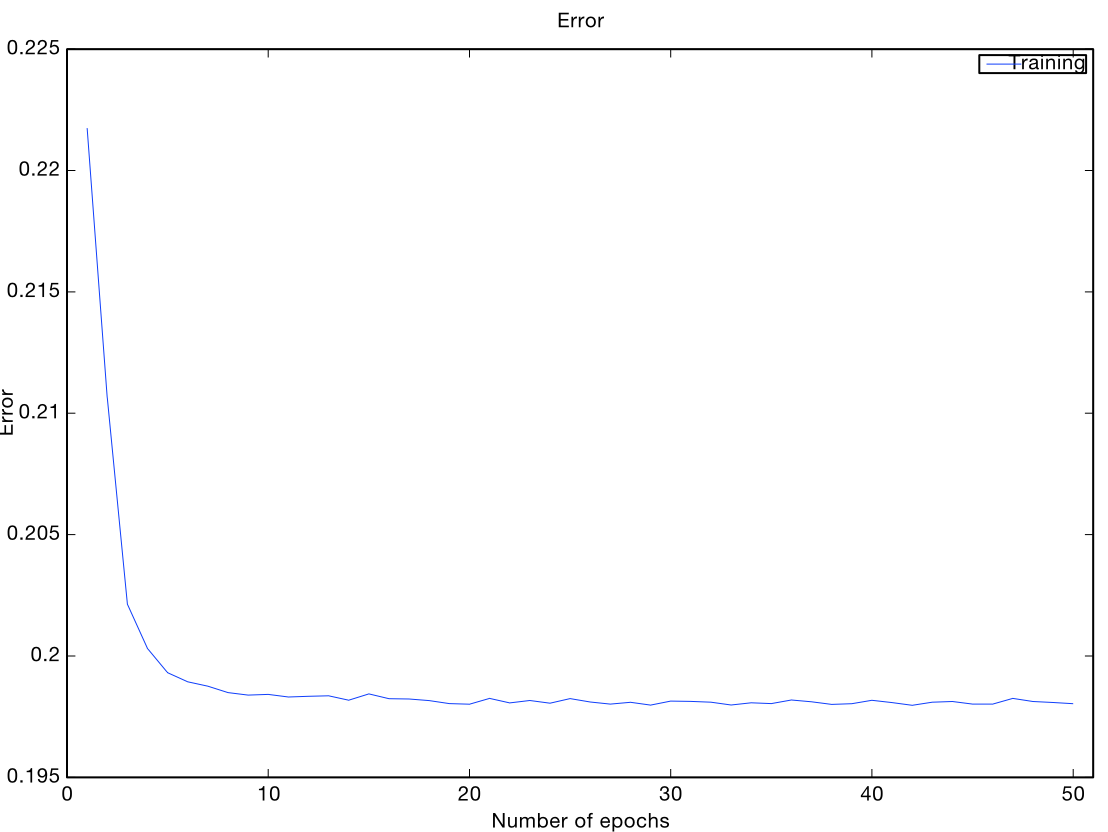
\includegraphics[scale=0.4]{3-5-7With12Error}

\item Here is a ROC plot\\





\end{itemize}

\subsection*{$\S$ Improved ANN}
For ANN, in general, the predition accuracy should improve when adding more hidden layer and/or hidden nodes. Thus we construct a improved ANN with 2 hidden layers, where there are 25 hidden nodes on the 1st hidden layer and 19 on the 2nd hidden layer. The activation functions are the same.
\begin{itemize}
\item Predicting Results Using 12 features
\begin{itemize}

\item Sigmoid function: Prediction Accuracy: 80.7%

\item Tanh function: ??

\end{itemize}
\item Here is an Error Rate plot\\
Need the 3D plot here


\item Here is a ROC plot\\
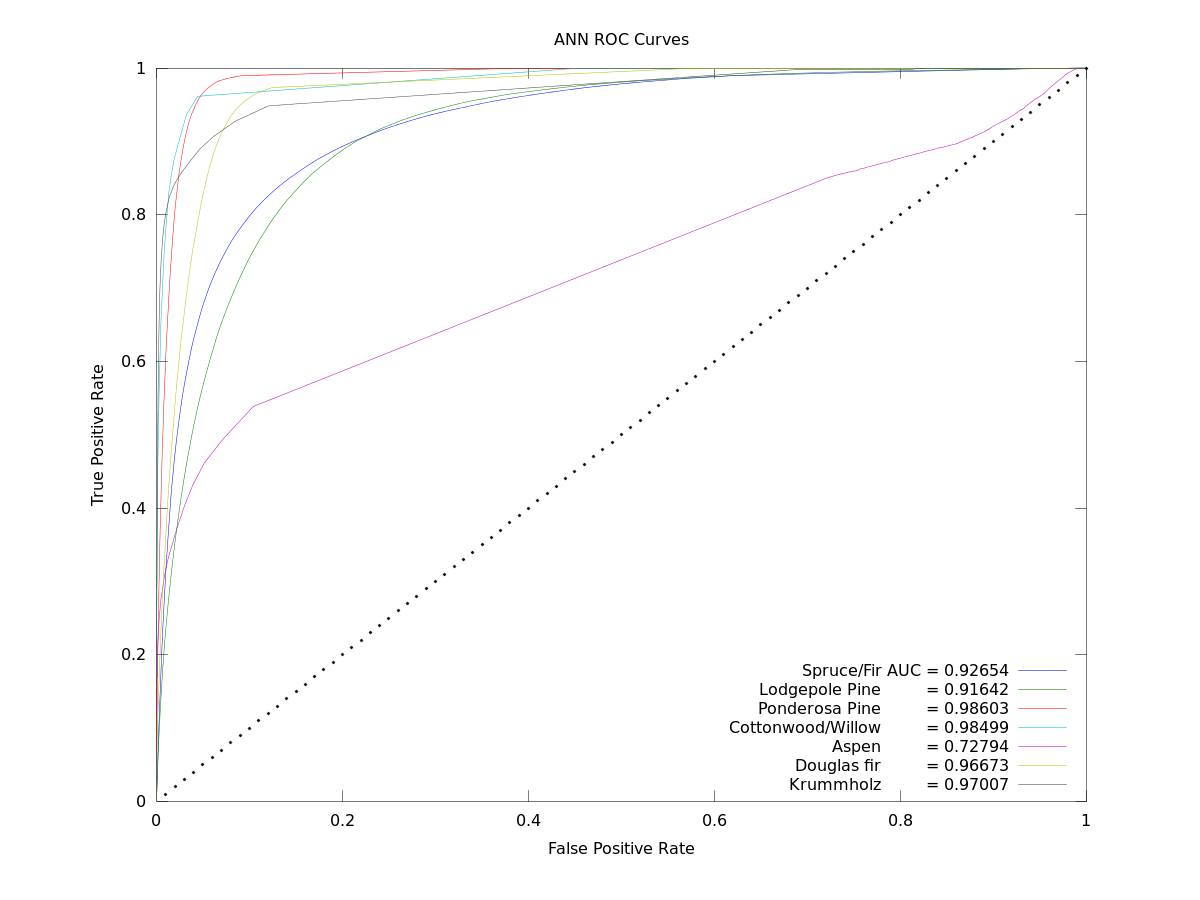
\includegraphics[scale=0.45]{ANNROCall}

\item abc\\
\begin{table} [h]
\caption{Confusion Matrix} % title of Table
\centering


\begin{tabular}{c c c c c c c}
\hline\hline %inserts double horizontal lines
Predicted1 & Predicted2 & Predicted3 & Predicted4 & Predicted5 & Predicted6& Predicted7 \\ [0.5ex] 
\hline % inserts single horizontal line
166919 & 42605 & 16 & 3 & 47 & 34 & 2216 \\
28706 & 250128 & 2821 & 8 & 310 & 996 & 330 \\
22 & 3140 & 30817 & 196 & 0 & 1579 & 0 \\
0 & 11 & 1671 & 863 & 0 & 202 & 0 \\
471 & 7176 & 288 & 0 & 1529 & 29 & 0 \\
124 & 4303 & 8558 & 110 & 1 & 4271 & 0 \\
5031 & 518 & 0 & 0 & 0 & 0 & 14961 \\
\hline % inserts single horizontal line
\end{tabular}
\end{table}


\end{itemize}

\subsection*{$\S$ Feature Selected ANN}
Instead of using all 12 features, we decide to use less feature which are relatively independent to each other. We first contructed a feature scatter plot to observe the dependency of features.\\
\\
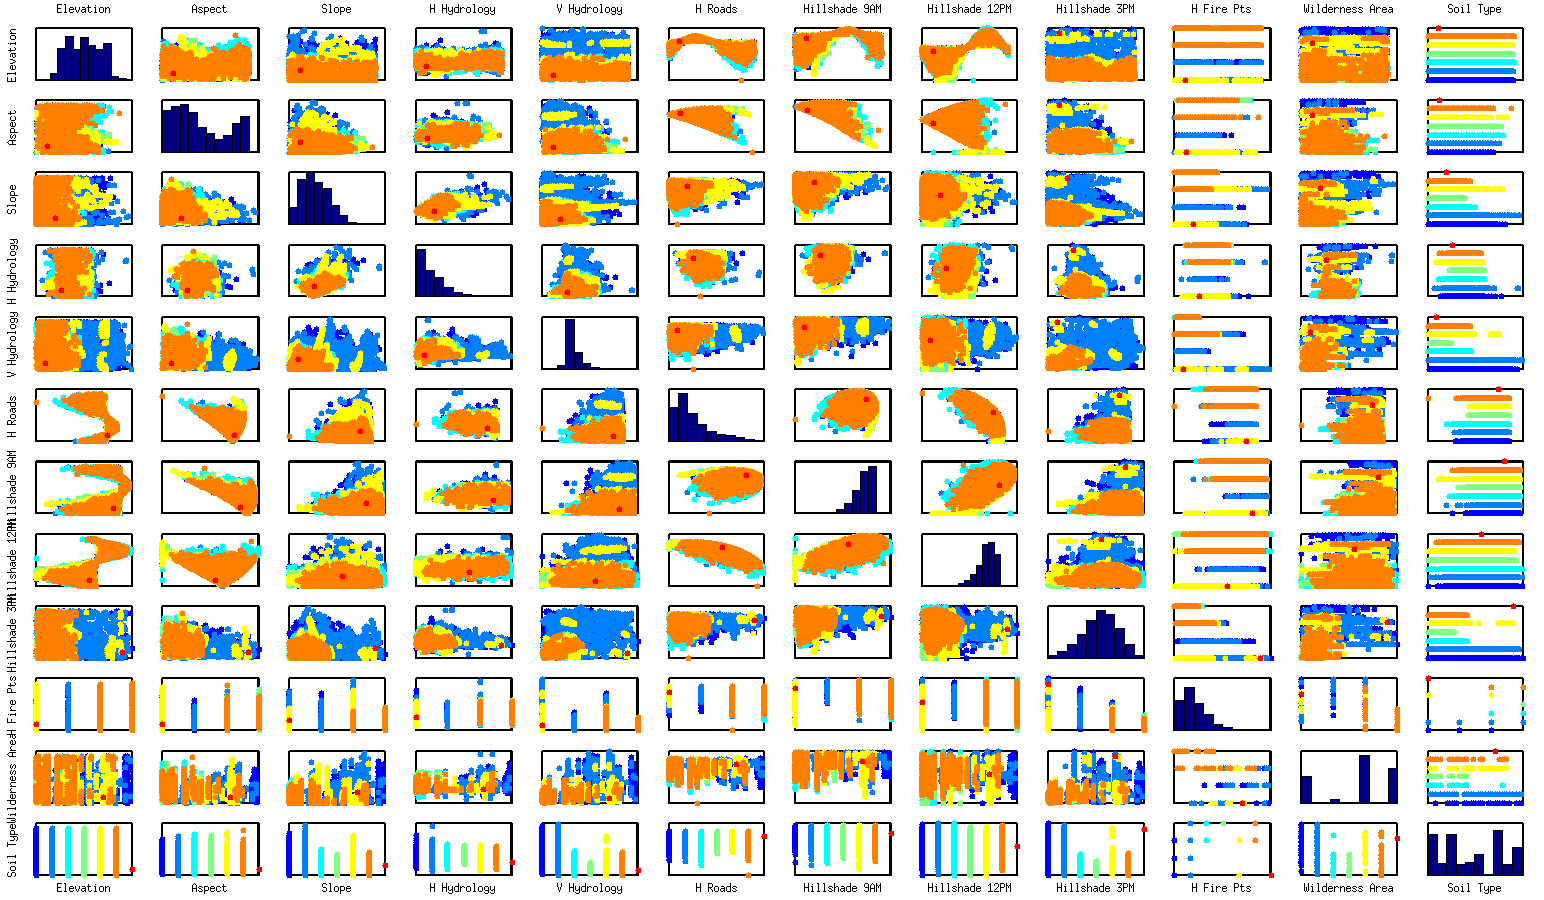
\includegraphics[scale=0.4]{featureScatterPlotMatrixHD}


The dependency and correlation of different features are not obvious. So we tested on a few cases, in which the prediction result aren't imporoved.

\begin{itemize}
\item 
\item 
\item 


\end{itemize}





\end{document}
